\section[Version control]{Version control with git}
\sectionframe{02}{Version control with git}
  {How do we keep every version, and see exactly what an agent changed?}
  {\faCodeBranch}

% ------------------------------------------------------------- what it is
\begin{frame}[source={Chacon \& Straub (2014), Pro Git, 2nd ed., git-scm.com/book}]{Version control: one folder, every version}
  \begin{columns}[T,onlytextwidth]
    \begin{column}{0.34\textwidth}
      \begin{ablock}[equal height group=vc,fontupper=\footnotesize]{Without}
        {\ttfamily\footnotesize splitting.py\\ splitting\_old.py\\ splitting\_v2\_final.py\\
         splitting\_v2\_final\_FIXED.py\\ results\_new2/\par}\vskip2mm
        Which version produced figure 3?
      \end{ablock}
    \end{column}
    \begin{column}{0.62\textwidth}
      \begin{dblock}[equal height group=vc,fontupper=\footnotesize]{With git}
        \centering
        \begin{tikzpicture}[x=1mm,y=1mm,
            commit/.style={circle,draw=udsblue,fill=white,line width=0.9pt,minimum size=3mm,inner sep=0pt},
            bcommit/.style={commit,draw=udsred},
            msg/.style={font=\scriptsize,text=udsdark,inner sep=0.6mm}]
          \draw[udsblue,line width=1pt] (0,0) -- (51,0);
          \draw[udsred,line width=1pt] (14,0) to[out=0,in=180] (23,9) -- (42,9) to[out=0,in=180] (51,0);
          \foreach \n/\x/\t in {a/0/random split,b/14/checks,m/51/merge} {
            \node[commit] (\n) at (\x,0) {};
            \node[msg,anchor=north] at (\n.south) {\t};
          }
          \foreach \n/\x/\t in {e/25/specimen folds,f/40/tests} {
            \node[bcommit] (\n) at (\x,9) {};
            \node[msg,anchor=south] at (\n.north) {\t};
          }
          \node[font=\scriptsize\bfseries,text=udsblue,anchor=east] at (-2.5,0) {main};
        \end{tikzpicture}\par\vskip1.5mm
        \raggedright\renewcommand\arraystretch{1.15}\setlength\tabcolsep{3pt}
        \begin{tabular}{@{}>{\bfseries}l l@{}}
          commit & a snapshot with a message, an author and a date\\
          diff   & what changed between two snapshots\\
          \textcolor{udsred}{branch} & a separate line of work, merged when ready\\
          remote & a copy on a server (GitHub): backup, sharing, review\\
        \end{tabular}
      \end{dblock}
    \end{column}
  \end{columns}
  \note{\textbf{6:00--7:10}\par
    Many of us keep versions as copies: splitting old, v2, final, fixed.\par
    After a few months nobody knows which copy produced a figure.\par
    Version control replaces the copies with one folder and its history.\par
    Git stores a snapshot of the project each time you commit, with a message, an author and a
      date; a diff shows what changed between two snapshots.\par
    A branch is a separate line of work, for an experiment or for an agent's task, merged back
      when it is ready.\par
    A remote such as GitHub holds a copy of the history on a server: a backup, a way to share,
      and the place where changes are reviewed.\par
    There a branch comes back as a pull request: a request to merge it, with its diff open for
      review before it reaches main.}
\end{frame}

% ------------------------------------------------------- learning curve
\begin{frame}[fragile,source={Chacon \& Straub (2014), Pro Git, 2nd ed., git-scm.com/book · Microsoft (2026), VS Code docs: Source control}]{Getting started takes five commands}
  \edef\colgap{\the\dimexpr0.04\textwidth\relax}
  \begin{columns}[T,onlytextwidth]
    \begin{column}{0.55\textwidth}
\begin{terminal}[basicstyle=\ttfamily\fontsize{7.2}{9.2}\selectfont]{terminal}
$ git init              # once: start the history
$ git status            # what has changed?
$ git add src/ tests/   # choose what goes in
$ git commit -m "Split by specimen"
$ git log --oneline     # the history so far
\end{terminal}
      \vskip1mm
\begin{codefile}[style=sh,basicstyle=\ttfamily\fontsize{7.2}{9.2}\selectfont]{.gitignore}
data/          # raw and derived data stay out
.venv/         # environments are rebuilt, not stored
*.ckpt         # model checkpoints
.env           # secrets
.claude/worktrees/  # agent worktrees
\end{codefile}
    \end{column}
    \begin{column}{0.41\textwidth}
      \begin{tikzpicture}
        \node[anchor=south west,inner sep=0pt,draw=udsgreylight,line width=0.4pt] (img) at (0,0)
          {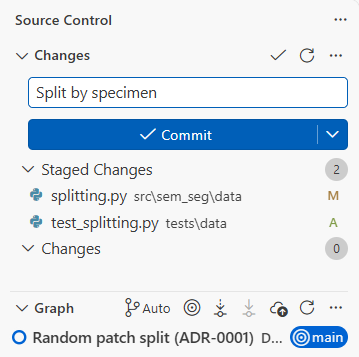
\includegraphics[height=36mm]{assets/screens/vscode-scm.png}};
        % each control, labelled with the command it replaces
        \begin{scope}[x={(img.south east)},y={(img.north west)}]
          \foreach \y/\t in {0.683/commit,0.521/add,0.412/status,0.057/log}
            \draw[udsgreymid,line width=0.5pt] (1,\y) -- ++(2.5mm,0)
              node[right,inner sep=0.6mm,font=\ttfamily\scriptsize,text=udsdark] {git \t};
        \end{scope}
      \end{tikzpicture}\par\vskip1mm
      {\scriptsize VS Code's Source Control panel does the same with clicks.\par}\vskip2mm
      % the arrow spans the gap between the columns (0.04 of the text width), so it starts at the
      % edge of .gitignore; drawn by the box itself, it also lands right in the notes thumbnails
      \begin{panel}[colback=redtint,borderline west={1.2mm}{0pt}{udsred},left=3.5mm,fontupper=\footnotesize,
          overlay={\draw[flow] ([xshift=-\colgap]frame.west) -- (frame.west);}]
        data, environments and secrets do not belong in the history
      \end{panel}
    \end{column}
  \end{columns}
  \note{\textbf{7:10--8:10}\par
    The learning curve is shorter than its reputation.\par
    Five commands cover daily use: start the history once, check what changed, choose what goes
      into the next snapshot, commit it with a message, and look at the history.\par
    VS Code's Source Control panel does the same with buttons: here two files are staged, the
      message is typed, one click on Commit, and the graph below is the history.\par
    A .gitignore file keeps out what does not belong in the history: data, environments, which
      are rebuilt from their description, model checkpoints, secrets, and the worktrees that Claude
      Code creates.\par
    Branches and merges can come later.}
\end{frame}

% ------------------------------------------------------- git and agents
\begin{frame}[source={OpenAI (2026), Agent approvals and security; Non-interactive mode · Anthropic (2026), Claude Code checkpointing}]{Why an agent needs version control}
  \begin{columns}[T,onlytextwidth]
    \begin{column}{0.66\textwidth}
      \begin{tikzpicture}
        \node[anchor=south west,inner sep=0pt,draw=udsgreylight,line width=0.4pt] at (0,0)
          {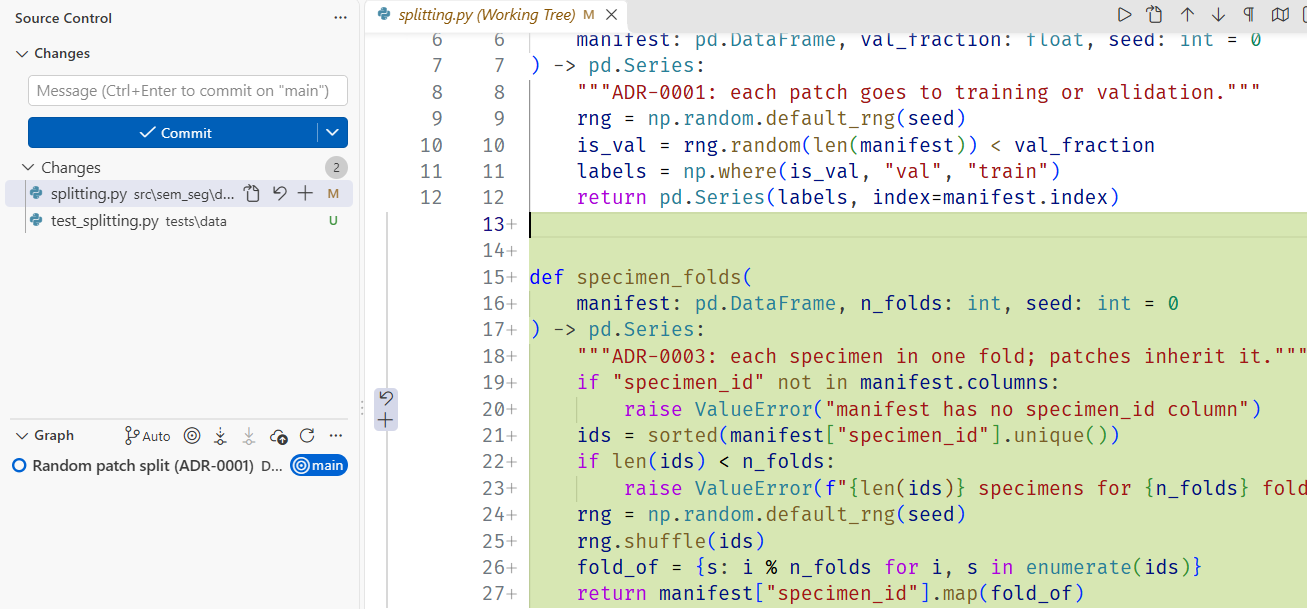
\includegraphics[width=\linewidth]{assets/screens/vscode-git.png}};
      \end{tikzpicture}\par\vskip1mm
      {\scriptsize An agent's change in VS Code's Source Control view: two files, every new line in green.\par}
    \end{column}
    \begin{column}{0.31\textwidth}
      \begin{tikzpicture}[x=1mm,y=1mm,
          commit/.style={circle,draw=udsblue,fill=white,line width=0.9pt,minimum size=3.4mm,inner sep=0pt},
          gitstep/.style={anchor=base west,inner sep=0pt,font=\footnotesize,text=udsdark,align=flush left,
            text width=38.6mm}]
        \useasboundingbox (0,0) rectangle (44.6,-52);
        % a checkpoint, the agent's uncommitted edits, then keep or discard them;
        % each label's first baseline sits 1 mm below its circle's centre
        \draw[udsblue,line width=0.9pt] (1.7,-1.9) -- (1.7,-14.4);
        \node[commit] at (1.7,-1.9) {};
        \node[gitstep] at (6,-2.9) {\textbf{checkpoint}\\commit before the agent starts};
        \node[commit,draw=udsred,dashed] (e) at (1.7,-14.4) {};
        \node[gitstep] at (6,-15.4) {\textbf{the agent's edits}\\read the diff, not the summary};
        \draw[udsblue,line width=0.9pt] (e.south) to[out=-90,in=180] (6,-27);
        \node[commit] at (7.7,-27) {};
        \node[gitstep,text width=33mm] at (11.6,-28)
          {\textbf{keep}\enspace\fn{git commit}\\{\color{udsgrey}undo later: \fn{git revert}}};
        \draw[udsgreymid,line width=0.9pt,dashed] (e.south) to[out=-90,in=180] (6,-38.6);
        \node[circle,fill=udsgreymid,text=white,inner sep=0pt,minimum size=3.4mm,font=\tiny]
          at (7.7,-38.6) {\faTimes};
        \node[gitstep,text width=33mm] at (11.6,-39.6)
          {\textbf{discard}\enspace\fn{git restore}\\{\color{udsgrey}the edits are lost}};
        \node[gitstep,text width=44.6mm,font=\footnotesize\bfseries,text=udsblue] at (0,-50.4)
          {one branch or worktree per task};
      \end{tikzpicture}
    \end{column}
  \end{columns}
  \note{\textbf{8:10--9:20}\par
    With git, an agent's work becomes a diff we can read before we accept it.\par
    Commit before the agent starts, so there is a checkpoint to return to.\par
    Read the diff itself, not the agent's summary of it: here, two files, every added line in
      green.\par
    Undo is one command: restore discards uncommitted changes for good, revert undoes a commit
      and keeps the history.\par
    A branch, or a separate worktree, per task keeps an agent's work apart from ours until it is
      reviewed.\par
    The tools assume all this.\par
    Codex checks at launch whether the folder is under version control, suggests read-only mode
      when it is not, and codex exec refuses to run outside a repository unless told
      otherwise.\par
    Claude Code can rewind its own file edits, but not files changed by shell commands, and its
      documentation says to keep using git.\par
    The workflow of section 6 commits each finished piece of work, and its review compares
      against a commit.}
\end{frame}

% ------------------------------------------------------------- worktrees
\begin{frame}[fragile,source={git documentation (2026), git-worktree · Anthropic Academy (2026) · DevToolLab (2026), worktrees guide}]{Worktrees: work in parallel, merge when done}
  \begin{columns}[T,onlytextwidth]
    \begin{column}{0.34\textwidth}
      \footnotesize
      \begin{itemize}\setlength\itemsep{1mm}
        \item one worktree per agent: its own folder, its own branch
        \item reviewed, then merged into \fn{main}
        \item one history, shared by every folder
        \item a branch is checked out in only one worktree
        \item \fn{main} changes only through merges
      \end{itemize}\vskip2mm
\begin{terminal}[basicstyle=\ttfamily\fontsize{7.2}{8.5}\selectfont]{terminal}
$ git worktree add ../folds \
    -b agent/folds
$ git worktree list
$ git worktree remove ../folds
\end{terminal}
    \end{column}
    \begin{column}{0.63\textwidth}
      \centering
      \begin{tikzpicture}[x=1mm,y=1mm,
          pill/.style={rounded corners=2mm,minimum height=4mm,inner xsep=2mm,inner ysep=0.4mm,
            font=\fontsize{7}{8}\selectfont\bfseries,text=white},
          dot/.style={circle,inner sep=0pt,minimum size=2.4mm},
          tie/.style={udsgreylight,dashed,line width=0.5pt},
          card/.style={draw=udsblue,fill=bluetint,line width=0.6pt,rounded corners=1mm,
            align=left,font=\scriptsize,inner xsep=1.6mm,inner ysep=1.2mm}]
        % branches first, so that dots and cards sit on top of them
        \draw[udsblue,line width=1pt] (68,3) to[out=135,in=270] (55,20) to[out=90,in=235] (68,31);
        \draw[udsblue,line width=1pt] (68,3) to[out=162,in=270] (27,20) to[out=90,in=200] (68,42);
        \draw[udsdark,line width=1.2pt,-{Stealth[length=2.4mm,width=1.8mm]}] (68,0) -- (68,46);
        % your own folder, on main
        \node[card,draw=udsred,fill=redtint,anchor=south] at (68,46.6)
          {{\color{udsred}\faFolderOpen}\ \textbf{\fn{sem-seg/}}\quad\faCodeBranch\ \fn{main}\quad\faUser\ you};
        % commits on main, on the right; the two merges in red
        \foreach \y/\t/\c in {3/commit/udsdark,14/your commit/udsdark,31/merge/udsred,42/merge/udsred} {
          \node[dot,fill=\c] at (68,\y) {};
          \draw[tie] (69.5,\y) -- (72,\y);
          \node[pill,fill=\c,anchor=west] at (72,\y) {\t};
        }
        % one worktree per branch: its folder, its branch, its agent
        \foreach \x/\n/\b in {55/1/folds,27/2/check} {
          \node[dot,fill=udsblue] at (\x,20) {};
          \draw[tie] (\x-1.5,20) -- (\x-3,20);
          \node[card,anchor=east] at (\x-3,20)
            {{\color{udsblue}\faFolderOpen}\ \textbf{\fn{../\b}}\\ \faCodeBranch\ \fn{agent/\b}\\ \faRobot\ agent \n};
        }
      \end{tikzpicture}
    \end{column}
  \end{columns}
  \note{\textbf{9:20--10:30}\par
    A worktree is a second working folder of the same repository, checked out on its own
      branch.\par
    Each card is one: a folder next to the repository, its branch, and the agent working in it;
      your own folder, sem-seg, is the main worktree on main.\par
    Both agents start from the same commit on main and work at the same time, while you keep
      committing on main in your own folder.\par
    When an agent's work is reviewed, its branch is merged into main: first one, then the
      other.\par
    All worktrees share one history, and git lets a branch be checked out in only one worktree
      at a time, so the agents get in neither each other's way nor yours.\par
    Three commands: add creates the folder and the branch, list shows them, remove deletes the
      folder once its branch is merged.}
\end{frame}

% ------------------------------------------- worktrees in the app and the terminal
\begin{frame}[source={Anthropic (2026), Claude Code docs: Desktop; Worktrees; CLI reference}]{Parallel sessions in the Claude app and the terminal}
  \begin{tikzpicture}[x=1mm,y=1mm,
      head/.style={anchor=north west,inner sep=0pt,font=\small\bfseries,text=udsdark},
      stage/.style={circle,fill=udsblue,text=white,inner sep=0pt,minimum size=5.6mm,font=\scriptsize},
      txt/.style={anchor=north west,inner sep=0pt,font=\footnotesize,text=udsdark,align=flush left,
        text width=61mm},
      mono/.style={anchor=west,inner sep=0pt,font=\ttfamily\fontsize{7}{8}\selectfont}]
    \useasboundingbox (0,0) rectangle (144,-55);
    \node[head] at (8,0) {Claude app};
    \node[head] at (83,0) {Terminal};
    \draw[udsgreylight,line width=0.4pt] (72,0) -- (72,-54.6);
    % the app: Worktree on under the prompt box (screenshot), with a red box on the button
    \node[anchor=north west,inner sep=0pt,draw=udsgreylight,line width=0.4pt] (app) at (8,-4.6)
      {
\includegraphics[width=61mm]{assets/screens/claude-app-worktree.png}};
    \begin{scope}[shift={(app.south west)},x={($(app.south east)-(app.south west)$)},
        y={($(app.north west)-(app.south west)$)}]
      \draw[udsred,line width=1.1pt] (0.552,0.01) rectangle (0.809,0.35);
    \end{scope}
    % the terminal: the session's own branch, as Claude Code shows it
    \fill[termbg,rounded corners=1.2mm] (83,-4.6) rectangle (144,-19.04);
    \foreach \c [count=\i] in {termdot1,termdot2,termdot3} \fill[\c] (83.4+\i*2.3,-7.2) circle (0.7);
    \node[inner sep=0pt,font=\ttfamily\fontsize{7}{8}\selectfont,text=termdim] at (113.5,-7.2)
      {claude --worktree specimen-folds};
    \draw[white!18!termbg,line width=0.4pt] (83,-9.8) -- (144,-9.8);
    \node[mono,text=termfg] at (85.6,-12.9) {! git branch --show-current};
    \node[mono,text=termfg] at (85.6,-16.4) {\phantom{! }└ worktree-specimen-folds};
    \draw[udsred,line width=1.1pt] (84.6,-10.9) rectangle (124.4,-18.4);
    \node[anchor=north west,inner sep=0pt,font=\scriptsize,text=udsgrey] at (8,-20.6)
      {\textbf{Worktree}: ``Work in an isolated copy of the repository''};
    \node[anchor=north west,inner sep=0pt,font=\scriptsize,text=udsgrey] at (83,-20.6)
      {the session runs on its own branch};
    % one session, start to end: the same four stages, with their icons, in both columns
    \foreach \x in {2.8,77.8} {
      \draw[udsgreylight,line width=1.2pt] (\x,-28.7) -- (\x,-51.5);
      \foreach \y/\icon in {-28.7/\faPlay,-36.3/\faFolderOpen,-43.9/\faClone,-51.5/\faFlagCheckered}
        \node[stage] at (\x,\y) {\icon};
    }
    \node[txt] at (8,-25.4) {\textbf{+ New} or Ctrl+N, then \textbf{Worktree}\\
      {\scriptsize\color{udsgrey}off by default, or on per saved environment}};
    \node[txt] at (83,-25.4) {\fn{claude -w specimen-folds}\\
      {\scriptsize\color{udsgrey}first time: trust the folder once}};
    \node[txt] at (8,-33.0) {\fn{.claude/worktrees/<name>/}\\
      \textcolor{udsblue}{\faCodeBranch}\ \fn{claude/<name>}};
    \node[txt] at (83,-33.0) {\fn{.claude/worktrees/specimen-folds/}\\
      \textcolor{udsblue}{\faCodeBranch}\ \fn{worktree-specimen-folds}};
    \node[txt] at (8,-40.6) {next task: the same again\\
      {\scriptsize\color{udsgrey}the sessions run side by side}};
    \node[txt] at (83,-40.6) {another terminal, another name\\
      {\scriptsize\color{udsgrey}another agent}};
    \node[txt] at (8,-48.2) {\textbf{Create PR}, merge, \textbf{Archive}};
    \node[txt] at (83,-48.2) {exit};
  \end{tikzpicture}
  \note{\textbf{10:30--12:40}\par
    Each session can run in its own worktree, from the Claude app or from the terminal.\par
    In the app: New or Ctrl+N, then turn on Worktree under the prompt box; it is off by default,
      so without it the agent edits your own checkout.\par
    A saved environment can switch it on for every session; Settings, Claude Code, sets the
      worktree location and the branch prefix.\par
    In the terminal: the flag worktree, or w, with a name; the first time, run claude once and
      trust the folder.\par
    Either way each session gets its own folder under .claude/worktrees and its own branch, so the
      agents run side by side.\par
    App sessions end with a pull request, a merge and Archive; uncommitted changes are kept for
      about thirty days.\par
    Leaving a terminal session removes an unchanged worktree and asks about a changed one.}
\end{frame}
